\documentclass[../main.tex]{subfiles}

\begin{document}
Para la realización de este apartado vamos a seguir el esquema de un fichero xml, el cual, tiene una estructura basada en el siguiente formato. 

\begin{figure}[h]
    \centering
    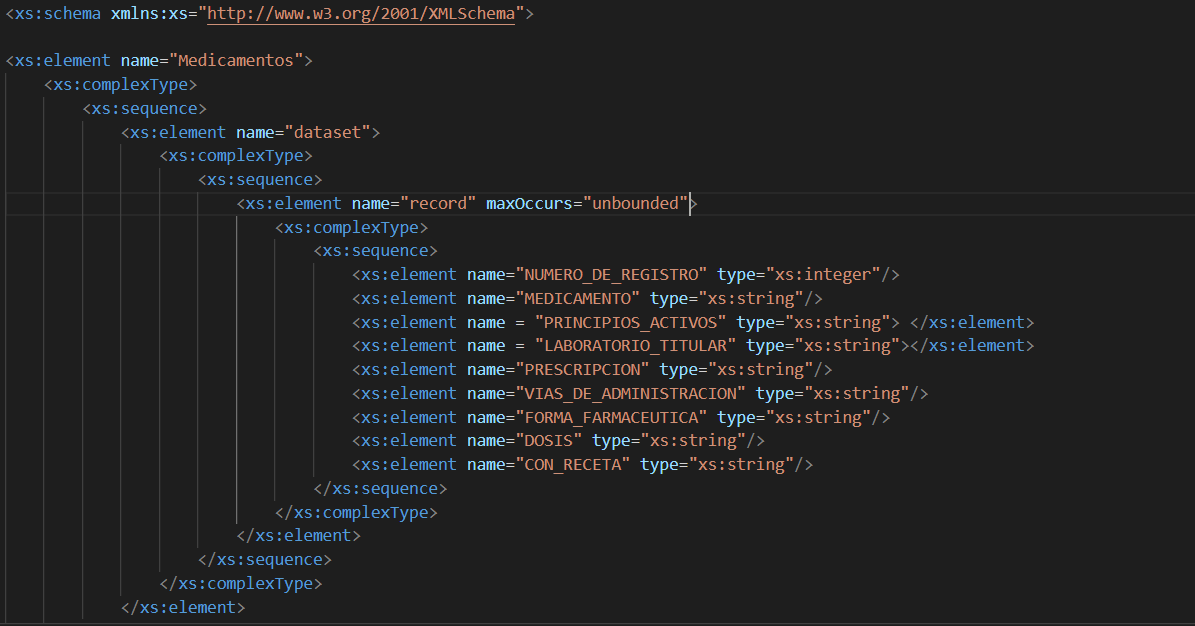
\includegraphics[scale=0.8]{images/schema.PNG}
    \caption{XML schema}
    \label{fig:mesh1}
\end{figure}




\subsection{Consula XQuery 1}

La primera consulta va a consistir en buscar en archivo xml todos los \textbf{medicamentos} con su \textbf{número de registro} y el \textbf{nombre de medicamentos} con un principio activo llamado \textbf{lacosamida} y con una \textbf{dosis de 200mg}. 

\lstset{language=HTML}
\begin{lstlisting}
       xquery version "3.1";
<html>
    <head>
        <tittle>Medicamentos con Lacosamida </tittle>
    </head>
<body>
<table border="1">
<tr>
    <td>Numero de registro</td>
    <td>Nombre del medicamento</td>
</tr>
    {
    for $b in doc("medicamentos.xml")//record
    where contains(data($b//PRINCIPIOS_ACTIVOS),"LACOSAMIDA") and contains(data($b//DOSIS),"200")
    return 
        <tr><td>{data($b//NUMERO_DE_REGISTRO)}</td><td>{$b//MEDICAMENTO}</td></tr>
    }
</table>
</body>
</html>
\end{lstlisting}

\begin{figure}[h]
    \centering
    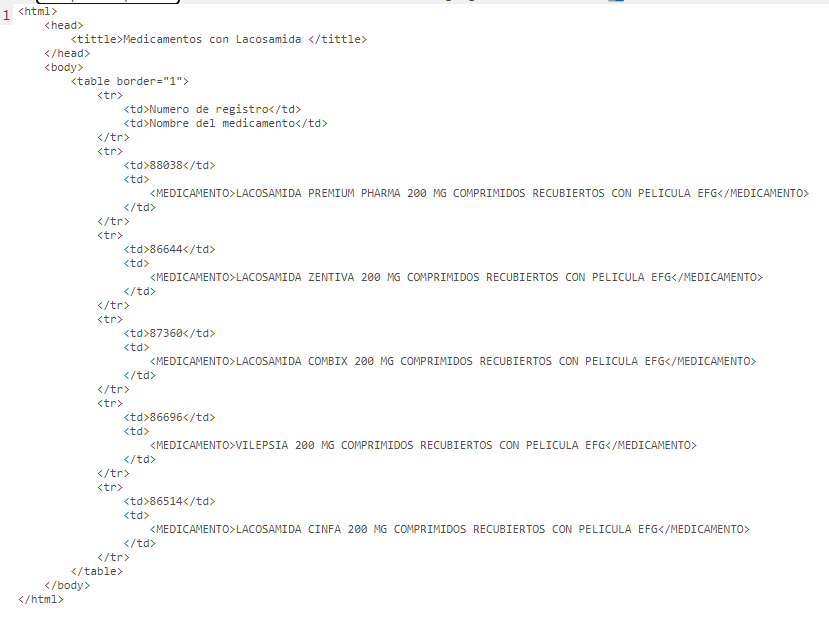
\includegraphics[scale=0.8]{images/xquery_1_output.PNG}
    \caption{Tabla en codigo hmtl de la primera consulta}
    \label{fig:mesh1}
\end{figure}
\newpage
\begin{figure}[h]
    \centering
    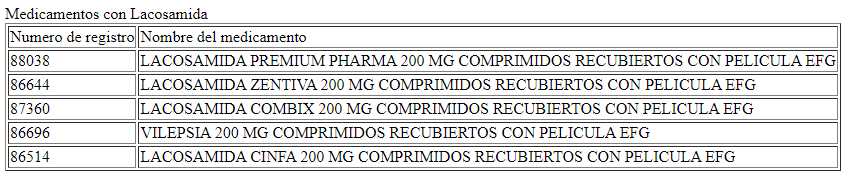
\includegraphics[scale=0.8]{images/xquery_1_html.PNG}
    \caption{Tabla de la primera consulta}
    \label{fig:mesh1}
\end{figure}

\newpage

\subsection{Consulta XQuery 2}
La segunda consulta XQuery que se ha realizado consiste en realizar una tabla en HTML que muestre ordenados \textbf{alfabéticamente} todos los medicamentos que sean \textbf{comprimidos recubiertos con película} y tengan una \textbf{dosis de 500 mg}.


\begin{lstlisting}
xquery version "3.1";
<html>
    <head>
        <tittle> Medicamentos con forma farmeceutica "Comprimido recubierto con pelicula" y dosis de 500mg ordenados alfabéticamente </tittle>
    </head>
    
    <body>
        <table border="1">
        <tr>
            <td>Numero de Registro</td>
            <td>Nombre del medicamento</td>
        </tr>
        {
            for $med in doc("medicamentos.xml")//record
            where contains(data($med//FORMA_FARMACEUTICA), "COMPRIMIDO RECUBIERTO CON PELICULA") and contains(data($med//DOSIS), "500 mg")
            order by $med//MEDICAMENTO
            return 
                <tr> 
                    <td> 
                        {data($med//NUMERO_DE_REGISTRO)}
                    </td>
                    <td>
                        {data($med//MEDICAMENTO)}
                    </td>
                </tr>
        }
        </table>
</body>
</html>

\end{lstlisting}

Una vez realizada esta XQuery, se puede observar el resultado de dos maneras diferentes. En primer lugar, la Figura 3 muestra el resultado mediante \textbf{código HTML} y en la Figura 4, se puede observar una \textbf{tabla} con todos los medicamentos que cumplen las condiciones de la consulta.

\begin{figure}[h]
    \centering
    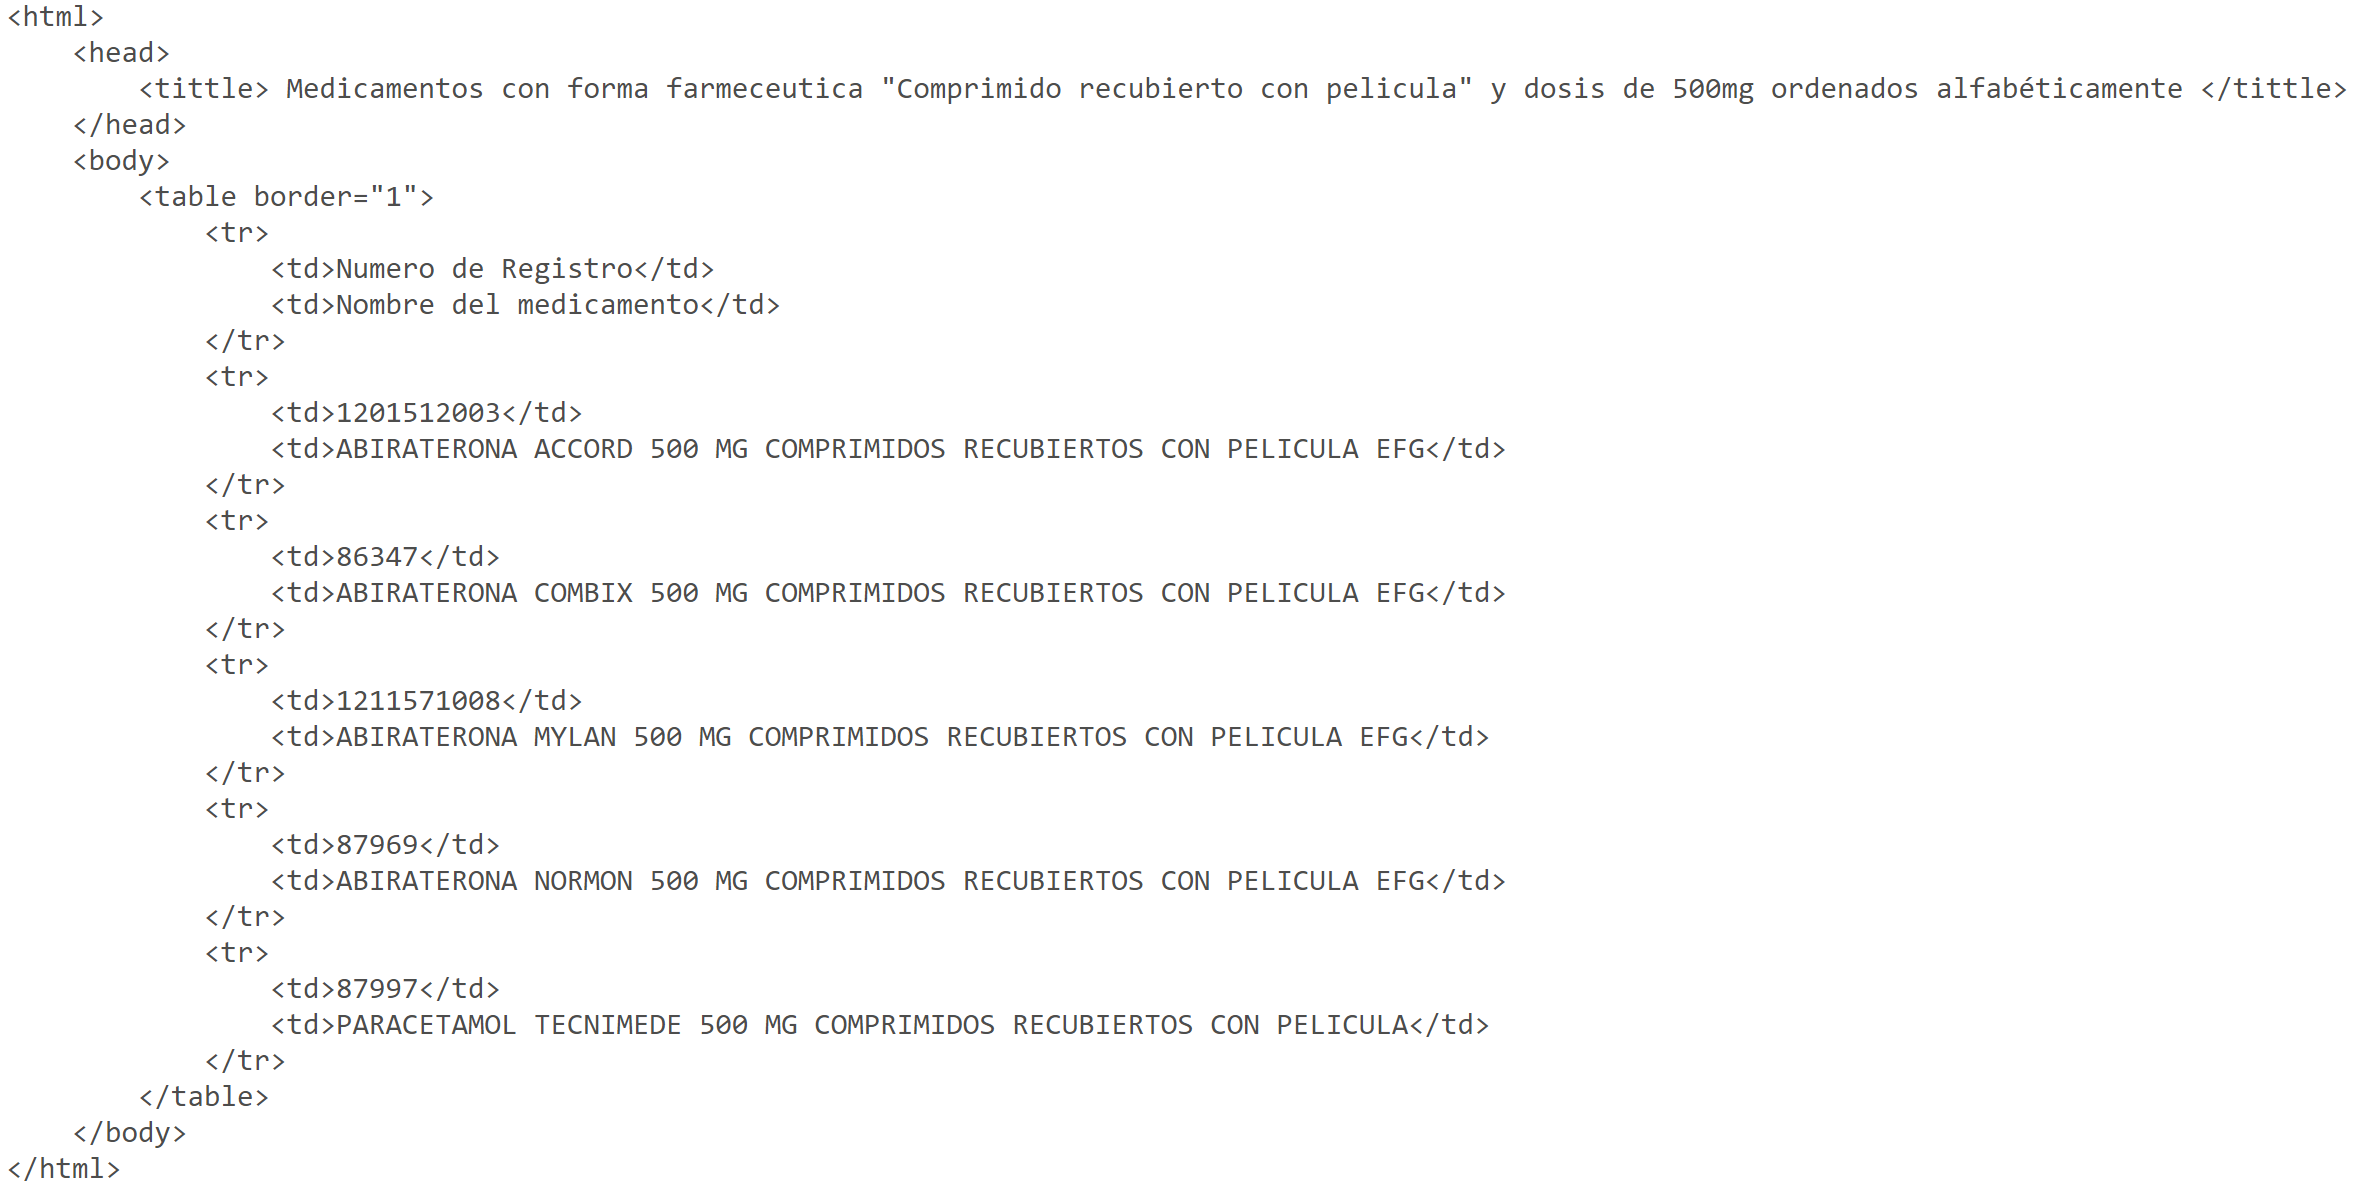
\includegraphics[scale=0.25]{images/xquery_2_html.png}
    \caption{Código en HTML de la segunda consulta}
    \label{fig:mesh1}
\end{figure}

\begin{figure}[h]
    \centering
    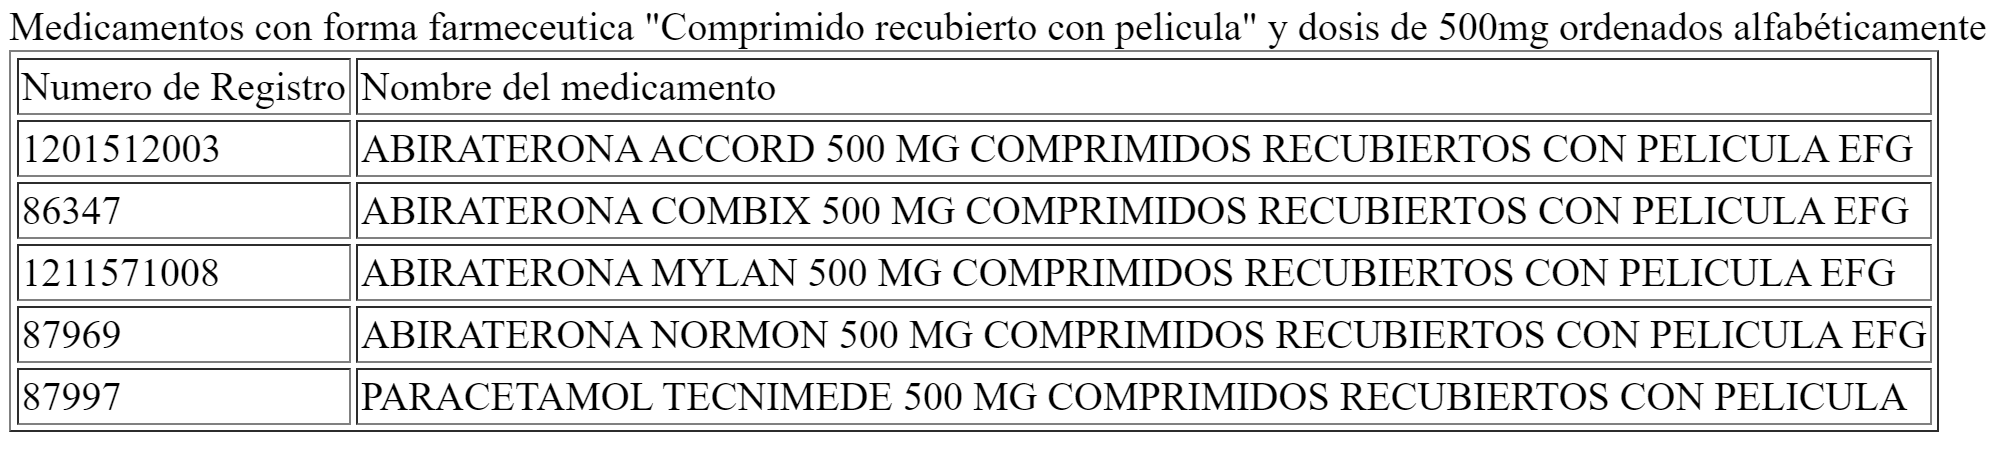
\includegraphics[scale=0.25]{images/xquery_2_output.png}
    \caption{Tabla resultante al realizar la segunda consulta}
    \label{fig:mesh1}
\end{figure}


\subsection{Consulta XQuery 3}
La tercera consulta XQuery consiste en filtar todos los medicamentos que se administren por vía oral y su nombre empiece por Aripiprazol.

\begin{lstlisting}
xquery version "3.1";
<html>
    <head>
        <tittle> Medicamentos con vía de administración oral y cuyo nombre empiece por aripiprazol </tittle>
    </head>
    
    <body>
        <table border="1">
        <tr>
            <td>Numero de Registro</td>
            <td>Nombre del medicamento</td>
        </tr>
        {
            for $med in doc("medicamentos.xml")//record
            where contains(data($med//VIAS_DE_ADMINISTRACION), "VIA ORAL") and starts-with(data($med//MEDICAMENTO),"ARIPIPRAZOL")
            return 
                <tr> 
                    <td> 
                        {data($med//NUMERO_DE_REGISTRO)}
                    </td>
                    <td>
                        {data($med//MEDICAMENTO)}
                    </td>
                </tr>
        }
        </table>
</body>

</html>

\end{lstlisting}

Evaluando la XQuery se pueden observar los dos tipos de outputs. En la Figura 5 se observa el \textbf{código HTML} resultante al realizar esta consulta y en la Figura 6 se observa la salida en forma de \textbf{tabla}.


\begin{figure}[h]
    \centering
    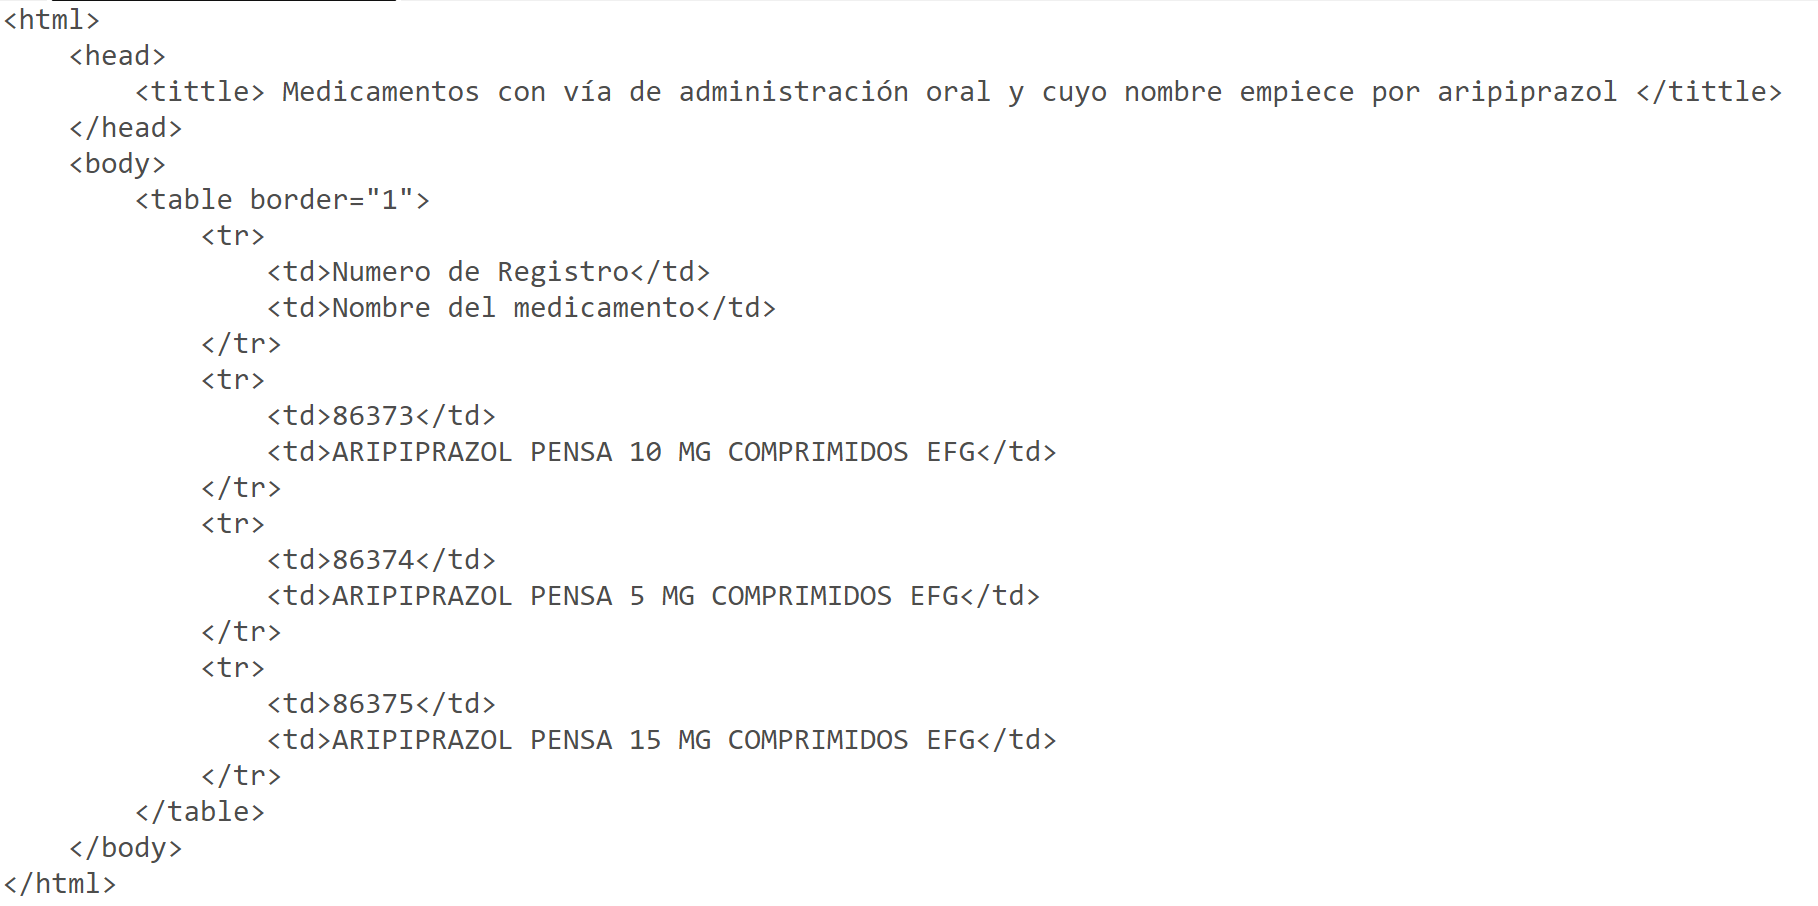
\includegraphics[scale=0.3]{images/xquery_3_html.png}
    \caption{Código en HTML de la segunda consulta}
    \label{fig:mesh1}
\end{figure}

\begin{figure}[h]
    \centering
    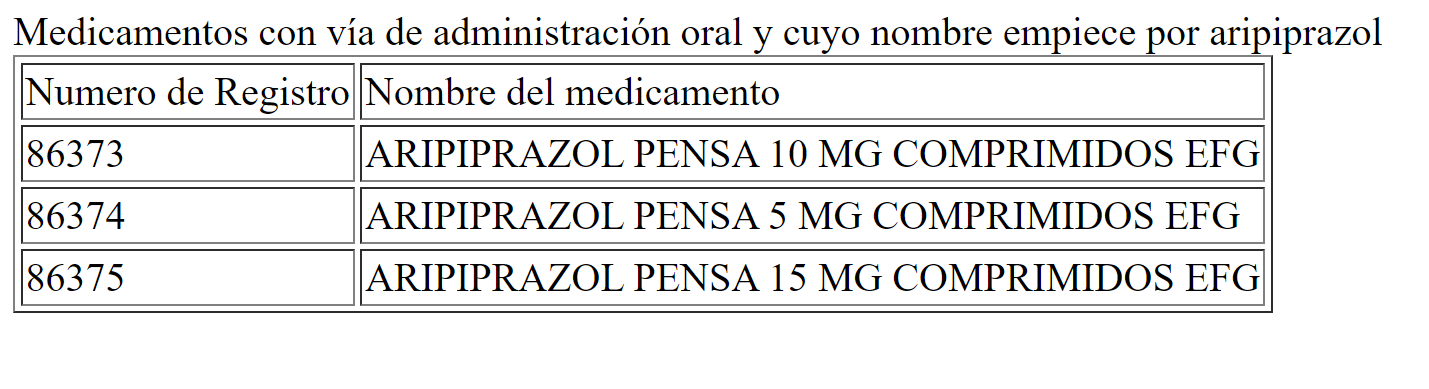
\includegraphics[scale=0.3]{images/xquery_3_output.png}
    \caption{Tabla resultante al realizar la segunda consulta}
    \label{fig:mesh1}
\end{figure}




\end{document}